\documentclass{article}
\textwidth=6in
\hoffset=0in
\voffset=0in

\usepackage{pgf}
\usepackage{tikz}
\usetikzlibrary{arrows,automata}
\usepackage[latin1]{inputenc}
\usepackage{ngerman}
\usepackage[a4paper, total={6in, 8in}]{geometry}
\usepackage{amsmath}
\usepackage{amssymb}
\usepackage{stmaryrd}
\usepackage{graphicx}
\usepackage{tikz}
\usetikzlibrary{automata, arrows}
\usepackage{pifont}
\usepackage{amssymb}
\usepackage{gensymb}
\usepackage[ampersand]{easylist}

\newcommand{\gap}{\ \\ \\}

% needs to be updated
\author{Max Springenberg, 177792}
\title{\
    ES "Ubungsblatt 1
    }
\setcounter{section}{1}
\date{}

\begin{document}

\maketitle
\newpage

\subsection{Nennen Sie mindestens zwei Anforderungen an Spezifikations- und 
            Modellierungssprachen f"ur eingebettete Systeme.}

Zu den in der Vorlesung vorgestelleten Anforderungen an Spezifiations- und 
    Modellierungssprachen f"ur eingebettete Systeme sind:\\

\begin{enumerate}
    \item Hierarchy
    \item Component-based design
    \item Timing
    \item Support design reactive systems
        \subitem event-handling/ state und error orientiertes Verhalten
\end{enumerate}

\subsection{}
\\

\subsection{}
(i)\\
\begin{tabular}{l|l|l|l}
    Zeit    &$e_1$   &$e_2$      & $a_1$ or $a_2$\\
    \hline
    0       &6       &0          & $a_1$\\
    1       &3       &2          & $a_1$\\
    2       &0       &4          & $a_2$\\
    3       &6       &0          & $a_1$\\
    4       &0       &4          & $a_2$\\
\end{tabular}\\
\gap
(ii)\\
\begin{tabular}{l|l|l|l}
    Time    &$e_1$   &$e_2$      & $a_1$, $a_2$ or ($a_1$ and $a_2$)\\
    \hline
    0       &9       &0          & $a_1$\\
    1       &6       &2          & $a_1$\\
    2       &3       &4          & $a_1$ and $a_2$\\
    3       &6       &2          & $a_1$\\
    4       &3       &4          & $a_1$ and $a_2$\\
\end{tabular}

\subsection{}
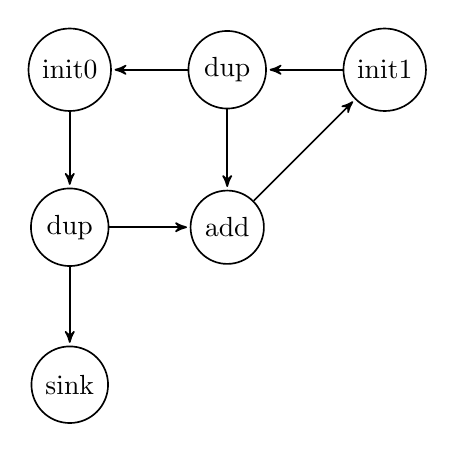
\begin{tikzpicture}[->,>=stealth',shorten >=1pt,auto,node distance=2.8cm,
                    semithick]
  %\tikzstyle{every state}=[fill=red,draw=none,text=white]

  \node[state] (init0)  at (0,0) {init0};
  \node[state] (init1)  at (4,0) {init1};
  \node[state] (dup0)   at (2,0) {dup};
  \node[state] (dup1)   at (0,-2) {dup};
  \node[state] (add)    at (2,-2) {add};
  \node[state] (sink)   at (0,-4) {sink};

  \path (init0) edge node {} (dup1)
        (init1) edge node {} (dup0)
        (dup0) edge node {} (init0)
               edge node {} (add)
        (dup1) edge node {} (add)
               edge node {} (sink)
        (add) edge node {} (init1);
\end{tikzpicture}
\end{document}
